\documentclass[times, twoside]{zHenriquesLab-StyleBioRxiv}
\usepackage{blindtext}
\usepackage[utf8]{inputenc}
\usepackage{graphicx}

\DeclareMathOperator*{\E}{\mathbb{E}}
\newcommand{\norm}[1]{\left\lVert #1 \right\rVert}

% Please give the surname of the lead author for the running footer
\leadauthor{Denovellis} 

\begin{document}

\title{A state space model for characterizing the trajectory dynamics of replay}
\shorttitle{Replay Dynamics}

% Use letters for affiliations, numbers to show equal authorship (if applicable) and to indicate the corresponding author
\author[1]{Eric L. Denovellis}
\author[2, 3]{Anna K. Gillespie}
\author[2, 3]{Michael E. Coulter}
\author[4]{Uri T. Eden}
\author[1, 2, 3, \Letter]{Loren M. Frank}


\affil[1]{Howard Hughes Medical Institute, University of California, San Francisco, San Francisco, California}
\affil[2]{Department of Physiology, University of California, San Francisco, San Francisco, California}
\affil[3]{Kavli Institute for Fundamental Neuroscience, University of California, San Francisco, San Francisco, California}
\affil[4]{Department of Mathematics and Statistics, Boston University, Boston, Massachusetts}

\maketitle

%TC:break Abstract
%the command above serves to have a word count for the abstract
\begin{abstract}
Representations of past or possible future experiences play a critical role in decision-making processes. The hippocampus is a brain region known to express these representations across multiple states, including during sharp-wave ripple (SWR) events where sets of hippocampal place cells can be activated in time-compressed sequences consistent with a rapid mental traversal of a path. Efforts to understand these representations typically make assumptions about the character and dynamics of the generative representations. As a result, we lack a clear picture of the nature and diversity of SWR representations. Here we develop a flexible state space model that uses a combination of discrete and latent states to describe the content and time evolution of SWR events. Application of this model reveals that a much larger proportion of SWR events contain coherent spatial content that previously reported, and that the dynamics of events span a surprisingly wide range. 

\end {abstract}
%TC:break main
%the command above serves to have a word count for the abstract

\begin{keywords}
Hippocampus | Replay | State Space
\end{keywords}

\begin{corrauthor}
%\texttt{loren{@}phy.ucsf.edu}
loren\at phy.ucsf.edu
\end{corrauthor}

\section*{Introduction}
The brain has the remarkable ability to retrieve representations of past events and generate representations of possible future events. These internal "generative" representations can be identified because the underlying neural activity patterns resemble those seen during actual events. In particular, an encoding model that relates neural firing to external covariates can be constructed during an experience, and this model can inverted to decode an internal representation of the covariates from the neural activity at a different time.

Mental events do not occur in the same time span as actual events; memories can be retrieved and used in less time than was required for the original experience, and mental simulations can span a series of actions more quickly than would be required to perform those actions. Consistent with this, generative representations can unfold rapidly. As a result, decoding generative representations requires making assumptions about their timescale and temporal structure, and these assumptions can limit the interpretation of the data. 

Hippocampal replay events are a prototypical example of a generative representation. As animals move through space, neurons in the hippocampus preferentially fire in at specific locations in an environment, and thus sets of cells can fire in sequence as the animal moves through a series of locations. When the animal is asleep or immobile, hippocampal cells can be reactivated during a "sharp-wave ripple" (SWR) event. A subset of SWRs contain sequential firing similar to that seen during a previous or potential future experience, and previous work has reported that these sequential firing events proceed at an average speed of ~10 meters / second, about 20x faster than the animal's usual movement speed \cite{DavidsonHippocampalReplayExtended2009}. 

Identifying these events typically involves multiple steps and assumptions about the nature of the event. First, an encoding model is constructed based on spiking activity during movement, most often using only spikes that have been clustered as single units (putative single neurons). Then, a subset of SWRs or events with high activity levels are selected based on an threshold for event size chosen by the experimenter. The spikes within these events decode the probability of position in overlapping or non-overlapping time bins whose size is also chosen by the experimenter. Finally, the most commonly used approach to detecting sequential replay involves fitting a line to the resulting set of probability distributions, which instantiates the assumption that the representations progress at a constant speed. A statistical test is then used to determining whether the fit is better than the fit to shuffled versions of the data.

While this approach identifies constant speed events, it does not consider events that are rejected by the statistical test, and the use of a fixed size temporal bin acts as a boxcar smoother that limits the potential movement speeds of the representation. The linear fit is also problematic, because it has the potential to reject real events that do not move at constant speeds. Moreover, there is now substantial evidence that a subset of these events express stationary representations, which are often excluded. In addition, these methods identify only a subset of events as containing content (typically somewhere between 10 and 45\% of the chosen events), and thereby provide little insight into the remaining majority of the events.

 Recognizing the problems with the linear fit, several studies have moved away from the constant velocity assumption, using the weighted mean or maximum of each posterior time bin and connecting each time bin with a line. For example, using this approach, Pfeiffer and Foster \cite{PfeifferAutoassociativedynamicsgeneration2015} found that replays can alternate between representing a single location and sequential spatial trajectories. On the other hand, Stella et al. \cite{StellaHippocampalReactivationRandom2019} found that replays are more spatially continuous, following Brownian diffusion dynamics. Both methods still used fixed time bins and neither took into account the uncertainty of the decoded estimates, making it hard to identify the source of the different conclusions.

An ideal approach to identifying and quantifying the dynamics of generative representations would circumvent these problems. It would use all of the available spiking data to yield the most accurate decoded positions. It would be applicable to either thresholded events or to all of the data to permit an unbiased assessment of the prevalence and nature of generative activity. It would use very small temporal bins (1 or 2 ms) to allow for very rapid representational movement and provide information about the certainty of the decoded estimates. It would be able to capture different types of movement dynamics, ranging from stationary to rapidly evolving to disorganized, and provide a statistical assessment of confidence for the dynamic. Finally, where assumptions are made, it would provide well defined parameters whose values can be explored systematically to understand their influence on the results.

We therefore developed a state space model of generative activity that achieves all of those goals. State space models are a well-understood, well-known statistical solution to the problems described above. By mathematically modeling the relationship between the data and latent dynamics, state space models make the assumptions of the model explicit and interpretable. Our model goes beyond previous approaches (refs) and characterizes represented trajectories as a mixture of three underlying patterns of dynamics: stationary trajectories, continuous trajectories that are many times the typical speed of the animal, and spatially fragmented trajectories. We show how this model can take advantage of clusterless decoding---which relates multiunit spike wave form features to position without spike sorting---giving us more information about the population spiking activity. We apply this model to data from 10 animals, focusing on SWR events to permit a direct comparison to previous work. We find that the vast majority of SWRs contain spatially coherent content. Surprisingly, while the expected high speed replay events were identified, the most common category of events expressed representations that moved at speeds consistent with real animal movement, suggesting that high speed replay is not the most common manifestation of generative activity. Our method provides a useful and powerful tool for understanding the dynamics of mental representations, and could be adapted for use in many brain areas. 

\section*{Results}
\begin{figure*}%[tbhp]
\centering
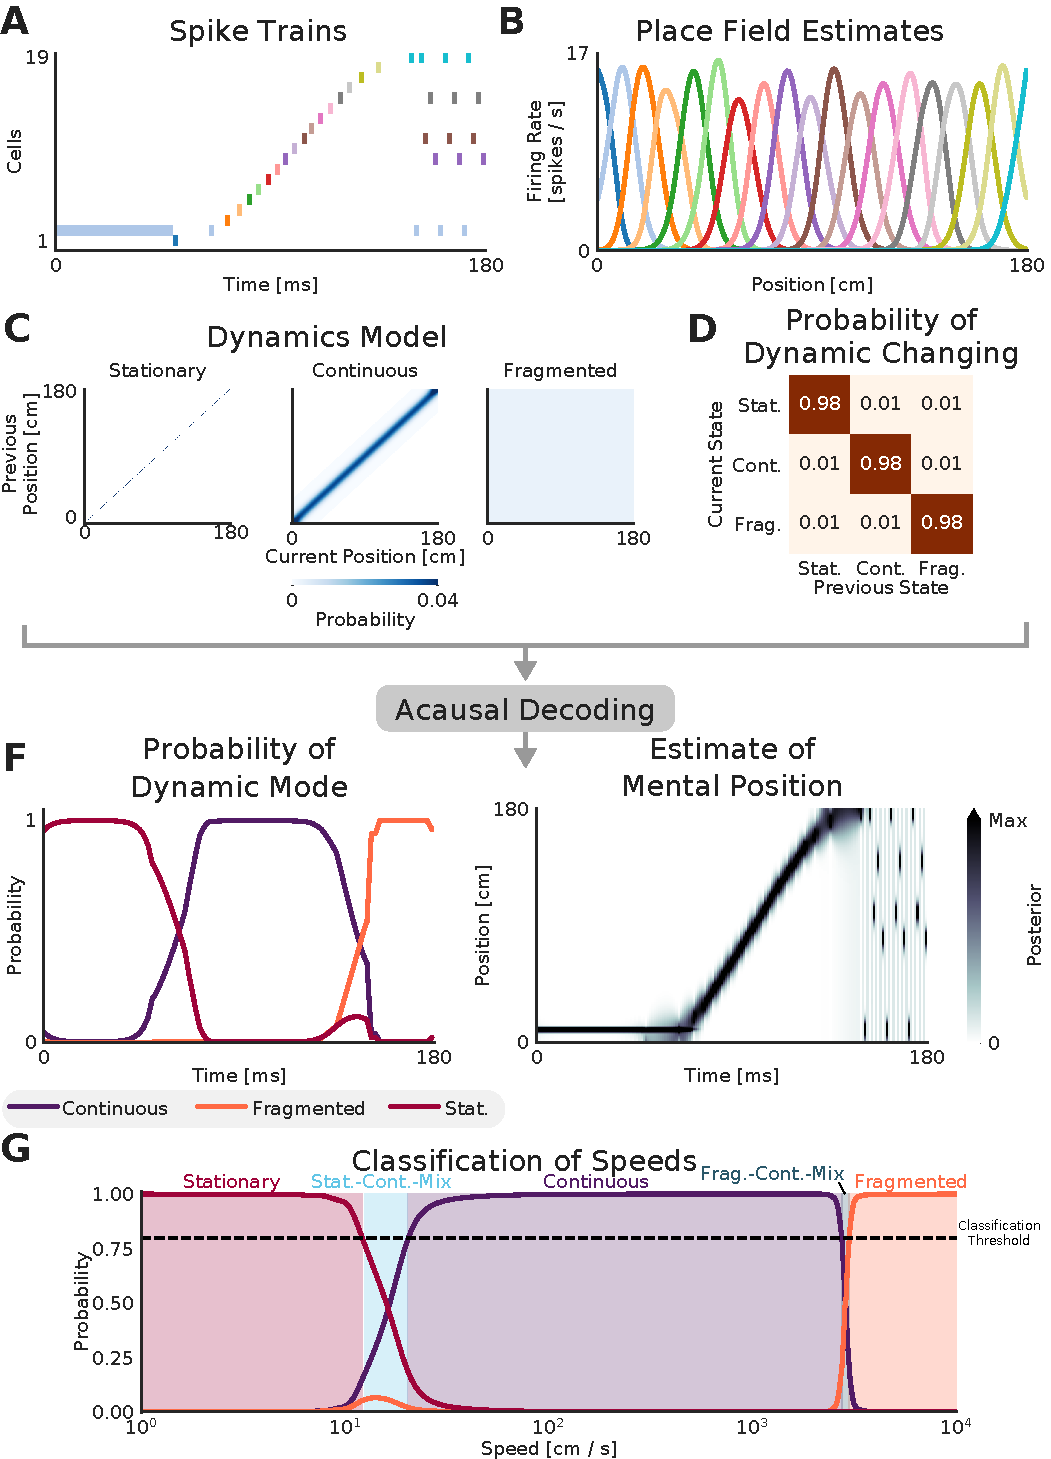
\includegraphics[width=0.80\linewidth]{figures/Figure1/Figure1_v4}
\caption{Components of the state space model and demonstration on simulated data. \textbf{(A)} 19 simulated place cells that exhibit three different sequence patterns. For the first third of time, one cell fires repeatedly, representing one stationary location. For the second third of time, the cells fire in sequence, representing a smooth continuous trajectory through space. For the last third cells fire in an incoherent pattern, representing a non-smooth fragmented trajectory through space. \textbf{(B)} Like the Bayesian Decoder, the state space model uses estimates of cells' place fields from when the animal is moving and combines them with the observed spikes in (A) to compute the likelihood of position for each time step. \textbf{(C)} This is combined with an explicit model of each dynamic state--which determines how latent position can change based on the posterior from the previous time step. In the stationary state, this is modeled as the identity matrix because the position remains the same. In the continuous state, the dynamics are modeled as a Gaussian random walk, meaning the next possible position is likely to be spatially close. In the fragmented state, the dynamics are modeled as uniform, meaning the next position is equally likely to be anywhere. Note that the dynamics displayed only reflect the within-state dynamics. \textbf{(D)} The probability of remaining in a particular state versus switching to another state. This is modeled as having a high probability of remaining in a particular state with a small probability of switching to one of the other dynamics at each time step. \textbf{(F)} The state space model uses the components in A-D over all time to decode the joint probability of latent position and dynamic state. The joint probability can be summarized by marginalizing over latent position (left panel) to get the probability of each dynamic state over time (lines). This can also be used to get an estimate of latent position over time (right panel). \textbf{(G)} The probability of each state given a particular constant speed trajectory. Each speed corresponds to a simulated spiking sequence at that speed. The lines correspond to the average probability of that state over the sequence. Dotted line represents the 0.8 classification threshold we use to classify each range of speeds and shaded regions correspond to the classification we have given the range of speeds.
}
\label{1}
\end{figure*}
\subsection*{Overview of the model}
In order to introduce and validate the model, we demonstrate how the model works on a simulated dataset (Figure \ref{1}). We simulated 19 Poisson spiking cells with Gaussian place fields on a 180 cm virtual linear track. Each place field has a 36 cm variance and a 15 Hz peak firing rate, which is spaced every 10 cm along the virtual track. We then apply our decoding algorithm to the spiking sequence in Figure \ref{1}A. For the first third of this sequence, a single place cell fires repeatedly, representing a single location. For the middle third of the sequence, the cells fire in sequential spatial order, representing a fast moving trajectory. For the last third, the cells fire in a incoherent spatial order. These firing patterns represent three different types of sequence dynamics, which we call stationary, continuous, and fragmented, respectively. The goal of our model is to characterize SWRs in terms of a mixture of these three dynamics at every time point.

Decoding the spiking sequence dynamics requires specifying two elements: the data model---how the spikes relate to position---and the dynamics model--how the position can change over time. For the data model, our decoder is the same as the Bayesian decoder. We compute an estimate of how each cell's firing rate varies over position (the place field, Figure \ref{1}B). This is used during decoding to compute the Poisson likelihood of position over time given the spiking sequence of interest. In contrast to the Bayesian decoder, we use small time bins (2 ms vs. 20 ms) because we are able to take advantage of the prior placed on the dynamics by the state space model. This allows us to detect changes on smaller time scales than would be possible with the Bayesian decoder.

Next, we specify a dynamics model for how latent position---the "mental" position of the animal represented by the cells---can evolve in each of these sequences (Figure \ref{1}C). We do this by defining a state transition matrix, which defines how the latent position can change from the previous time step. In the stationary dynamic, we expect latent position to not change between time steps, so we use an identity state transition matrix, which predicts the next position will be the same as the last position. In the continuous dynamic, we expect the latent position to be "spatially close" to the position in the previous time step, so we use a Gaussian random walk state transition matrix. This means that, for a given latent position, the probability of moving to another position is modeled by a Gaussian centered at that position and "spatially close" is defined by the variance of the Gaussian. In our case, since we are interested in identifying replays that move at speeds much faster than the animal's speed, we set this to 6.0 cm. This ensures that with a 2 ms time step, the latent position is 95\% likely to be within 4.90 cm of the previous latent position (or 24.5 m/s), consistent with replay speeds observed in previous studies \cite{DavidsonHippocampalReplayExtended2009, PfeifferAutoassociativedynamicsgeneration2015}. In the fragmented dynamic, we expect that the latent position can move to any available position instantaneously. We model this using a uniform state transition matrix, which makes all positions equally likely.

Finally, we specify how likely the dynamic is to persist in time versus changing to another dynamic (Figure \ref{1}D). In order to be conservative, we assume that each dynamic is likely to dominate for the duration of the SWR, with a small probability of switching to one of the other dynamics. Therefore, we set the probability of staying in a state to 0.98 for each 2 ms time step. Because the probability of changing dynamics follows a geometric distribution, this corresponds to an expected duration of 100 ms for staying in a particular state.

Once we have specified the data and dynamics model, we have fully specified the state space model. We use acausal decoding, meaning that we use all information from the past and future spikes, to estimate the joint posterior probability of position and dynamic state. With this, we can summarize the resulting posterior with two quantities: the mixture probability of each dynamic over time and the probability of position over time, irrespective of dynamic (Figure \ref{1}F, left and right plot respectively). From these two summaries, we can see that the model successfully captures the dynamics of the population spiking activity in Figure \ref{1}A. The probability of the stationary dynamic has high probability at the beginning of the simulated replay, reflecting the consistent spiking from one cell. This gives way to the continuous dynamic, reflecting the trajectory-like spiking from the population of cells. Then the fragmented dynamic dominates for the last third when the population spiking is not spatially coherent. We can also see that these three dynamics are reflected in the estimate of latent position of the animal.  Importantly, we get a much less variable estimate due to the correct specification of the dynamics.

One way to interpret the probabilities in our model is as a classifier of speeds of replay. To demonstrate this, we applied the model to simulated trajectories of increasing speed (Figure \ref{1}G), from 1 cm/s to 10,000 m/s. From this, we can see that not only are there regions of speed that correspond to our three dynamics being high probable (where we define highly probable to be over 0.8 probability), there are in-between speeds where two of the dynamics dominate with high probability; that is, the sum of two of the dynamics' probabilities is over 0.8. In this manuscript, we will refer to these as mixture dynamics. For example, when the stationary state has a probability of 0.6 and the continuous has a probability of 0.4, we call this a stationary-continuous mixture (light blue, Figure \ref{1}G). By using this classification scheme, we can characterize the speed or set of speeds in a replay by its dynamics.

In order to verify that the model was robust to the choice of probability of staying in a state, we decoded the spiking sequence in Figure \ref{1}A with different probabilities of staying in the same state versus switching to another state (Figure 1-Supplemental Figure 1). We found that for a large range of plausible probabilities of staying in one of the dynamics (0.9 - 0.9999), the model still correctly identified the dynamic with high probability.

\begin{figure*}%[tbhp]
\centering
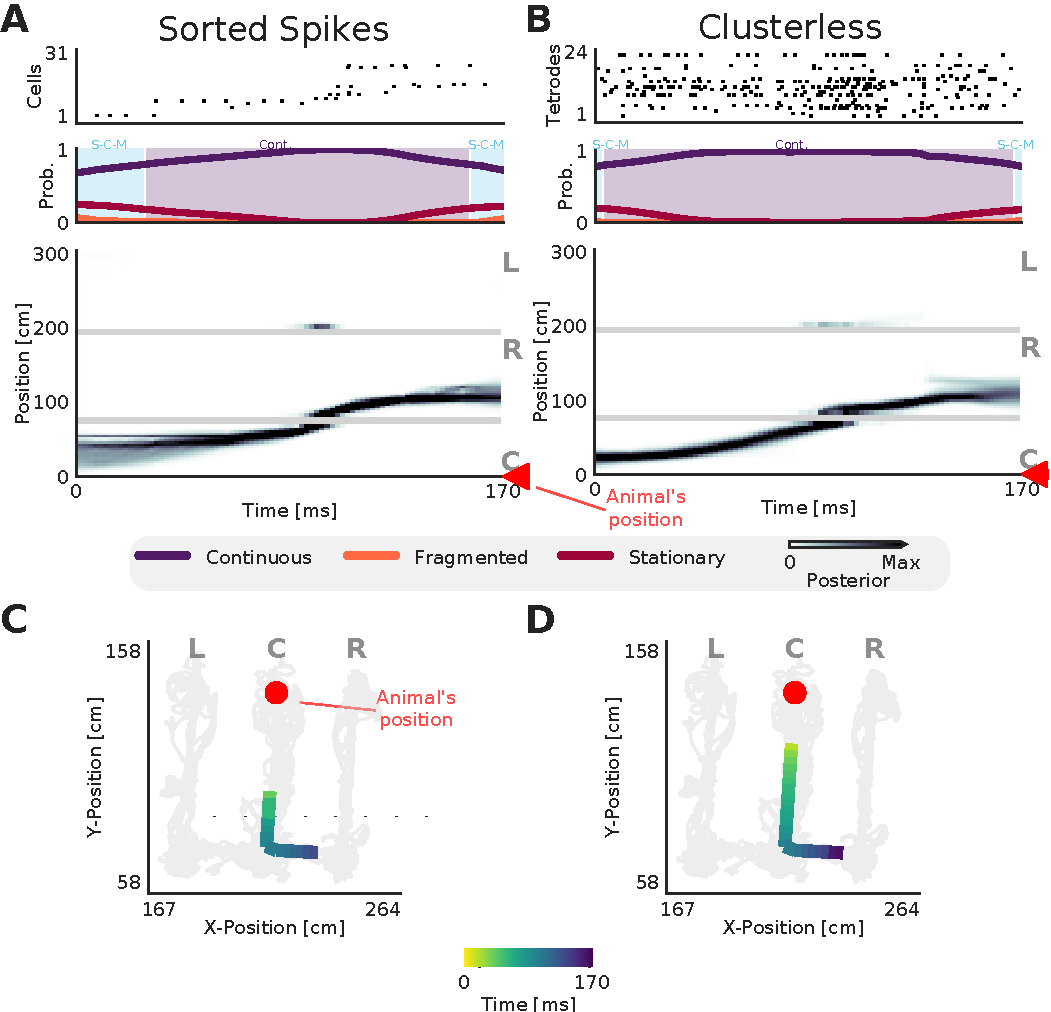
\includegraphics[width=0.80\linewidth]{figures/Figure2/Figure2_v4}
\caption{Demonstration of the state space model on real data using both sorted and clusterless spikes on the same SWR. \textbf{(A)} Decoding using sorted spikes (arranged top to bottom). In the top panel, 31 cells on a W-track ordered according to linearized position by their place field peaks. The second panel shows the probability of each dynamic over time as in Figure 1F. Shaded regions correspond to the speed classifications as in Figure 1G. The third panel shows the estimated probability of latent position over the course of the SWR as it travels down the center arm toward the right arm. L, R, C correspond to the position of the left, right and center wells respectively. The animal's position is indicated by the red triangle. \textbf{(B)} Decoding using clusterless spikes. The top panel shows multiunit spiking activity from each tetrode. Other panels have the same convention as(A).  \textbf{(C)} 1D MAP estimate of the latent position in (A) projected back into 2D. Color indicates time. The animal's position is denoted by the red circle. Light grey lines show the animal's 2D position over the entire epoch. L, R, and C correspond to the left, right and center well as in (A). \textbf{(D)} 1D MAP estimate of the latent position in (B) projected back into 2D. Figure conventions are the same as in (C).
}
\label{2}
\end{figure*}
\subsection*{The model finds known continuous replays with sorted and clusterless spikes}

\begin{figure*}%[tbhp]
\centering
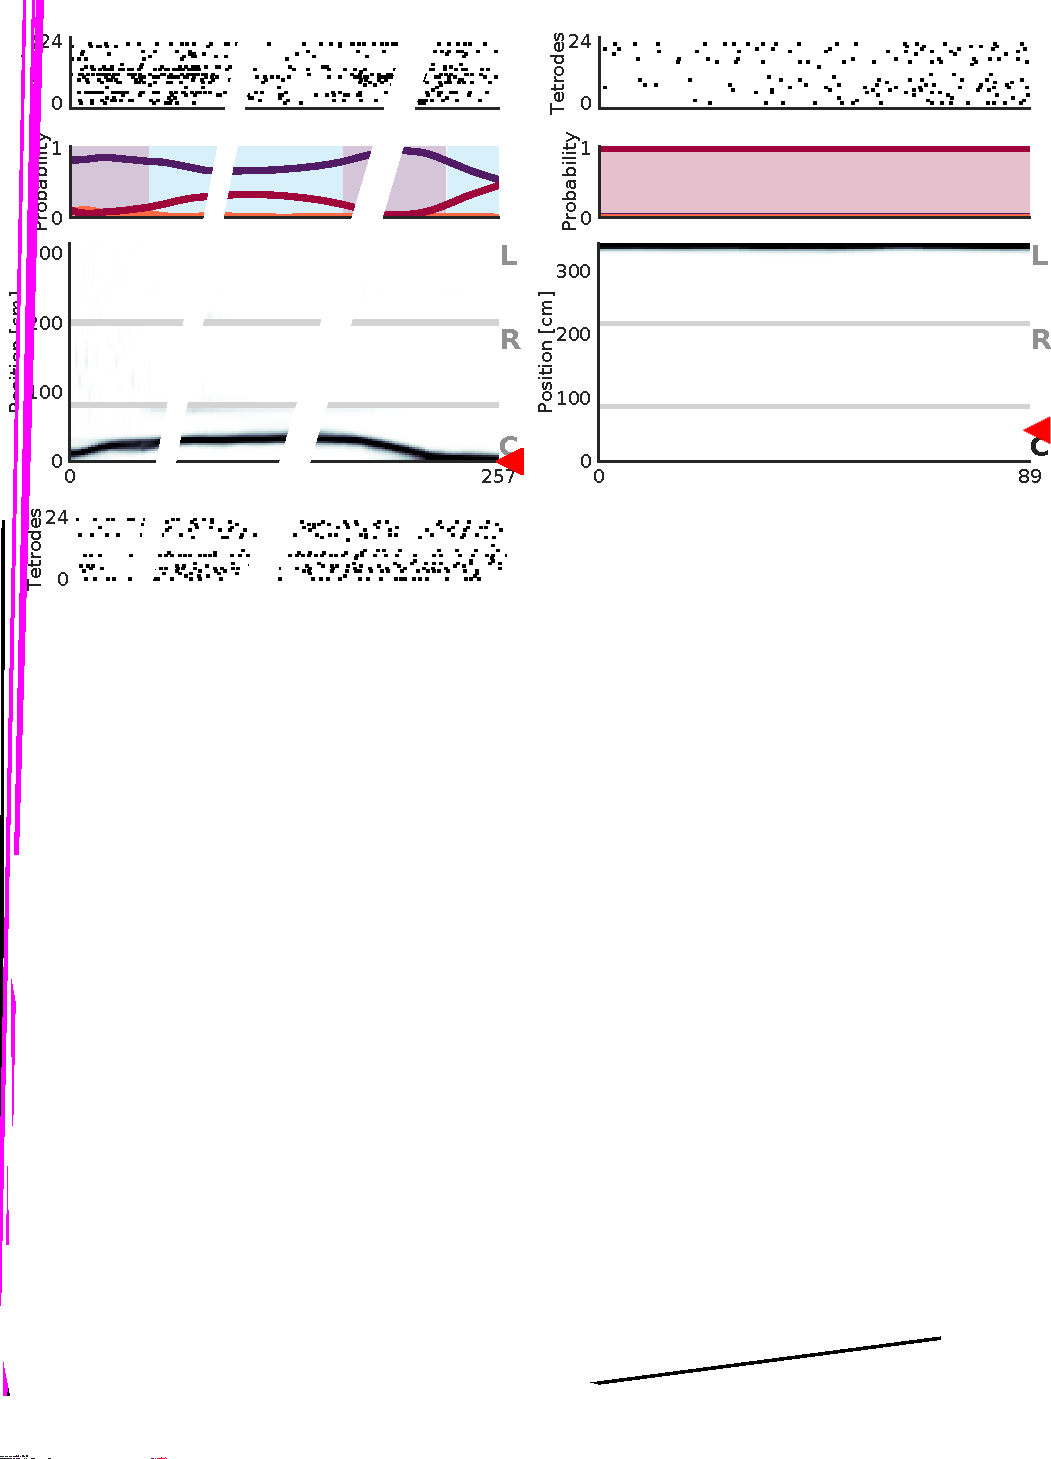
\includegraphics[width=0.80\linewidth]{figures/Figure3/Figure3_v4}
\caption{A-D. Four examples of replays that would not be well-characterized by using the Bayesian decoder. Figure conventions are the same as in Figure 2. \textbf{(A)} A replay that starts down the center arm away from the animal's position at the center well, slows down, and returns back. \textbf{(B)} A replay that stays at the left well for the entirety of the SWR while the animal is in the center arm. \textbf{(C)} A replay that begins stationary at the left well and then jumps to the middle of the right arm and proceeds up the right arm to the right well. \textbf{(D)} A replay that begins stationary at the left well, jumps to the center arm, proceeds away from the center well, jumps to the right arm, proceeds back toward the center well, and then becomes fragmented. \textbf{(E)} Percentage of SWRs in each epoch that has some content that falls into one of the categories (Stationary, Stationary-Continuous-Mix, Continuous, Fragmented-Continuous-Mix, or Fragmented). \textbf{(F)} Of the classified content, the percentage of SWRs in each epoch that have some Stationary, Stationary-Continuous-Mix, or Continuous content. \textbf{(G)} Of the classified content, the percentage of SWR in each epoch that has some Continuous content.
}
\label{3}
\end{figure*}

Next, we wanted to validate the model on real hippocampal data. We fit the place fields of 31 cells recorded in hippocampus while the rat was performing a spatial alternation task on a W-shaped track, and then applied the decoding algorithm to a SWR with clear sequential population activity (Figure \ref{2}A, top panel). We observed that the probability of being in the continuous dynamic is high throughout for this SWR, with the probability of being in a stationary state being slightly higher at the beginning and end of the SWR (Figure \ref{2}A, middle panel). Using our speed classification scheme, this means that the speed of the replay starts slower---as a mixture of continuous and stationary dynamics---and then speeds up and slows down again. This is also evident in the posterior probability of linear position over time. This shows that the replay travels down the center arm and up the right arm (Figure \ref{2}A, bottom panel). We can also see this when we project the maximum of the posterior of this trajectory to 2D (Figure \ref{2}C) to better see the spatial trajectory. Moreover, when we apply the same model using the 2D position of the animal, we get a similar result as when we used the 1D linearized position (Figure 2-Supplemental 1A).

One problem with using spikes from cells identified using spike sorting is that there is potentially a lot of information lost by determining the identity of each cell---many spikes are discarded because the spikes could not be uniquely assigned to one cell. Therefore, we wanted to use a method which directly relates spikes and their multiunit spike waveform features to position without spike sorting, which we call clusterless decoding. Clusterless decoding previously has been used to successfully identify theta sequences and replay sequences in the hippocampus (\cite{KloostermanBayesiandecodingusing2014, ChenTransductiveneuraldecoding2012,DengRapidclassificationhippocampal2016, KayConstantSubsecondCycling2020}). Here, if we apply it to the same SWR as the sorted spikes, we get similar decoding and classification of the sequence (Figure \ref{2}B, D), both with 1D linearized position and 2D position (Figure 2-Supplemental 1B). Note that, using clusterless decoding, the estimate of the posterior probability of position is much more narrow, indicating that there is more certainty in the true latent position at that time compared the corresponding posterior probability of position using sorted spikes (Figure \ref{2}D vs C).

\subsection*{The model finds replays with non-constant speed dynamics}
After validating our model on a single SWR, we then applied our decoding algorithm to hippocampal recordings from 10 animals performing the W-track spatial alternation task (tetrodes = [10, 24], brain areas = [CA1, CA2, CA3]; some data previously used in \cite{KarlssonAwakereplayremote2009}). We observed many replays that were classified as continuous throughout the entirety of SWR and likely would have been identified by the typical Bayesian Decoder (Figure 2-Supplemental 2A-C). However, we also observed replays that did not have this structure, but could be interpreted in terms of our model. For example, we observed trajectories that started in one direction and reversed back to the original position (Figure \ref{3}A, Figure 3-Supplemental 1B), trajectories that stayed in one position (Figure \ref{3}B), trajectories that jumped between arms (Figure \ref{3}C-D, Figure3-Supplemental 1A, E, F), and trajectories that remained spatially incoherent throughout the SWR (Figure3-Supplemental1D). Overall, we were able to classify 89\% ( 23382/26160) of SWRs as containing at least one of the five dynamics. To verify that this depended on the spatial receptive fields of cells in the hippocampus, we resampled position with replacement for two epochs, breaking the relationship between spiking and spatial information. There were far fewer SWR classified when spatial information was removed (XX fewer SWRs, CI [], p=0.XX for epoch 1, p=0.XX for epoch 2, Figure 3-Supplemental 2).

To better understand the distribution of dynamics during SWRs, we then asked what percentage of classified replays contained spatially coherent content---which we define as a SWR containing any times with stationary, stationary-continuous mixture, or continuous dynamics. We found that 22478 of 23382 or 96\% of SWR had some spatially coherent structure while 3353 of 23382 or 14\% had some spatially incoherent structure. This was consistent across animals (Figure \ref{3}F). We then asked what percentage of SWR contained continuous content, like would typically be analyzed when using the Bayesian decoder. We found that, consistent with previous reports, only 4511 of  23382 or 19\% of SWRs had some continuous content (Figure \ref{3}G). This highlights that much of the SWR replay content is missed when analyzing SWRs with the Bayesian decoder.

To verify that partitioning the data into spatially coherent and incoherent time segments by dynamic was meaningful, we quantified the cumulative spatial extent of the 95\% highest posterior density (HPD) values of the posterior linear position. Larger values of the cumulative HPD indicate the model is less certain about position, because the HPD values are spread out over more of the track at a given time point, whereas lower values indicate that the model is more certain about the estimate of position, because the HPD values are more concentrated and cover less of the track. For example, Figure \ref{4}A and B show two SWRs that were classified as having stationary and continuous dynamics, respectively. The bulk of the HPD values at each time step in these SWRs is concentrated on a small portion of the track and so the cumulative HPD is low throughout the SWRs. In contrast, the Figure \ref{4}C shows a SWR where the dynamics are fragmented and correspondingly, the HPD is much more spatially diffuse and the cumulative HPD is much higher. This can change over the time course of a SWR, as in Figure \ref{4}D, where the cumulative HPD is small for most of the SWR until the end, where the uncertainty of position becomes much higher. When we looked at the average cumulative HPD for each SWR by dynamic, we found a clear bi-modal split between spatially congruent dynamics and spatially incongruent dynamics (Figure \ref{4}E). For the spatially congruent dynamics, the cumulative HPD was much lower than the spatially incongruent dynamics (median XX cm, spatially congruent vs. median XX cm, spatially incongruent).

## Reminder: need colorbar and legend
\begin{figure*}%[tbhp]
\centering
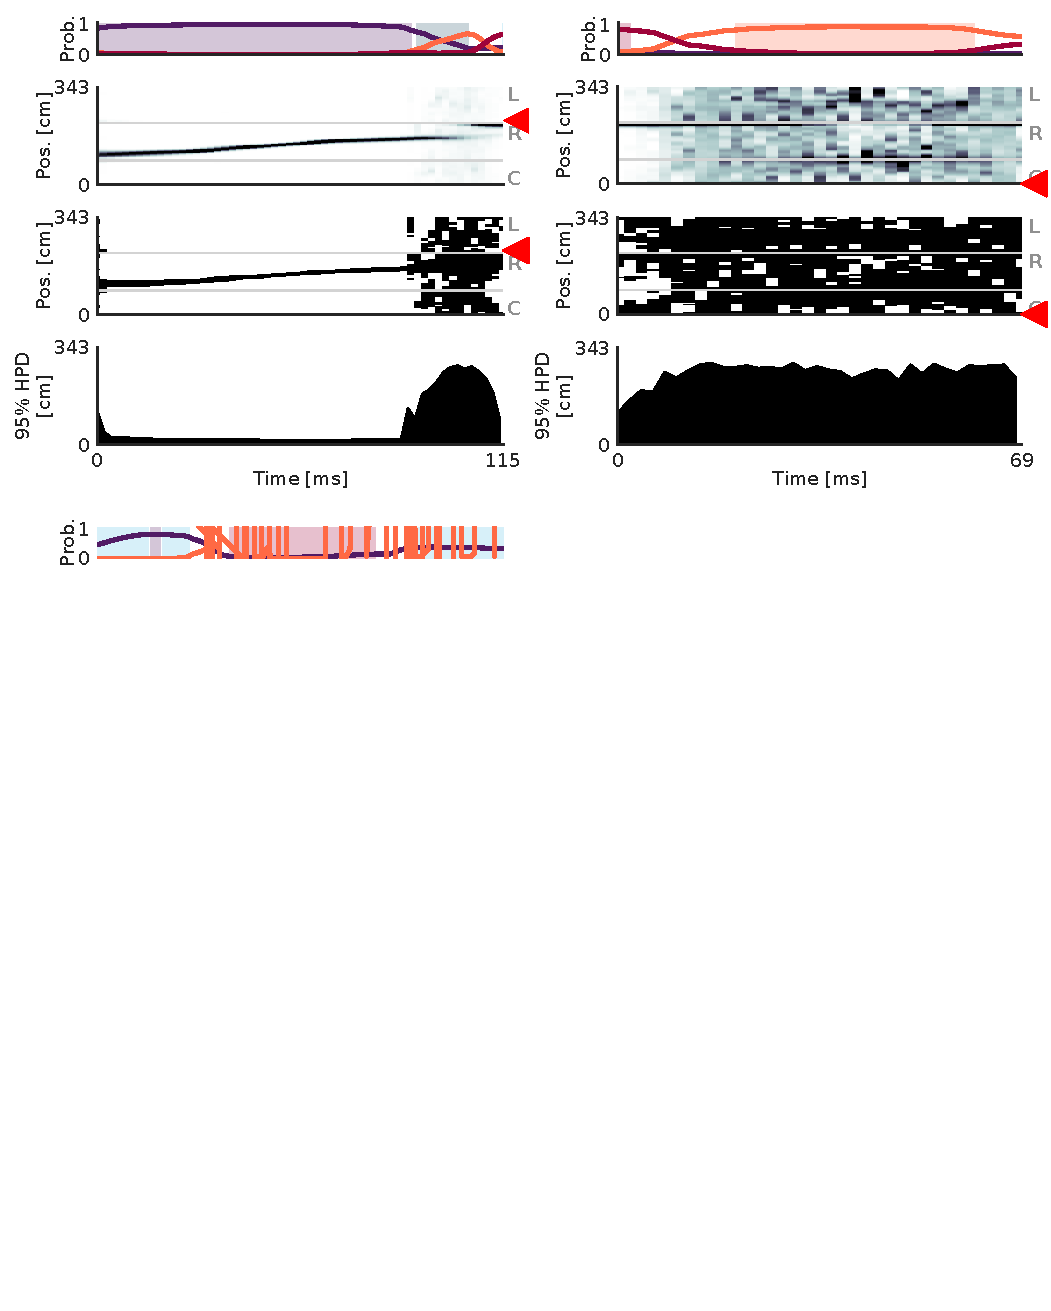
\includegraphics[width=0.80\linewidth]{figures/Figure5/Figure5_v2}
\caption{95 \% Highest Posterior Density of the Dynamics. \textbf{(A-D)}  Examples of the 95 \% Highest Posterior Density. Top panel. Probability of dynamic over time. Shading and labels indicates dynamic categories. 2nd panel. Posterior linear position over time. Red triangle indicates animal's position. 3rd panel. Black indicates the position bin is in the 95\% highest posterior density (HPD) values. 4th panel. Cumulative HPD. \textbf{(E)} Average Cumulative 95\% HPD for each dynamic category.}
\label{4}
\end{figure*}

\subsection*{Many replay trajectories have slower movement speeds}
\begin{figure*}%[tbhp]
\centering
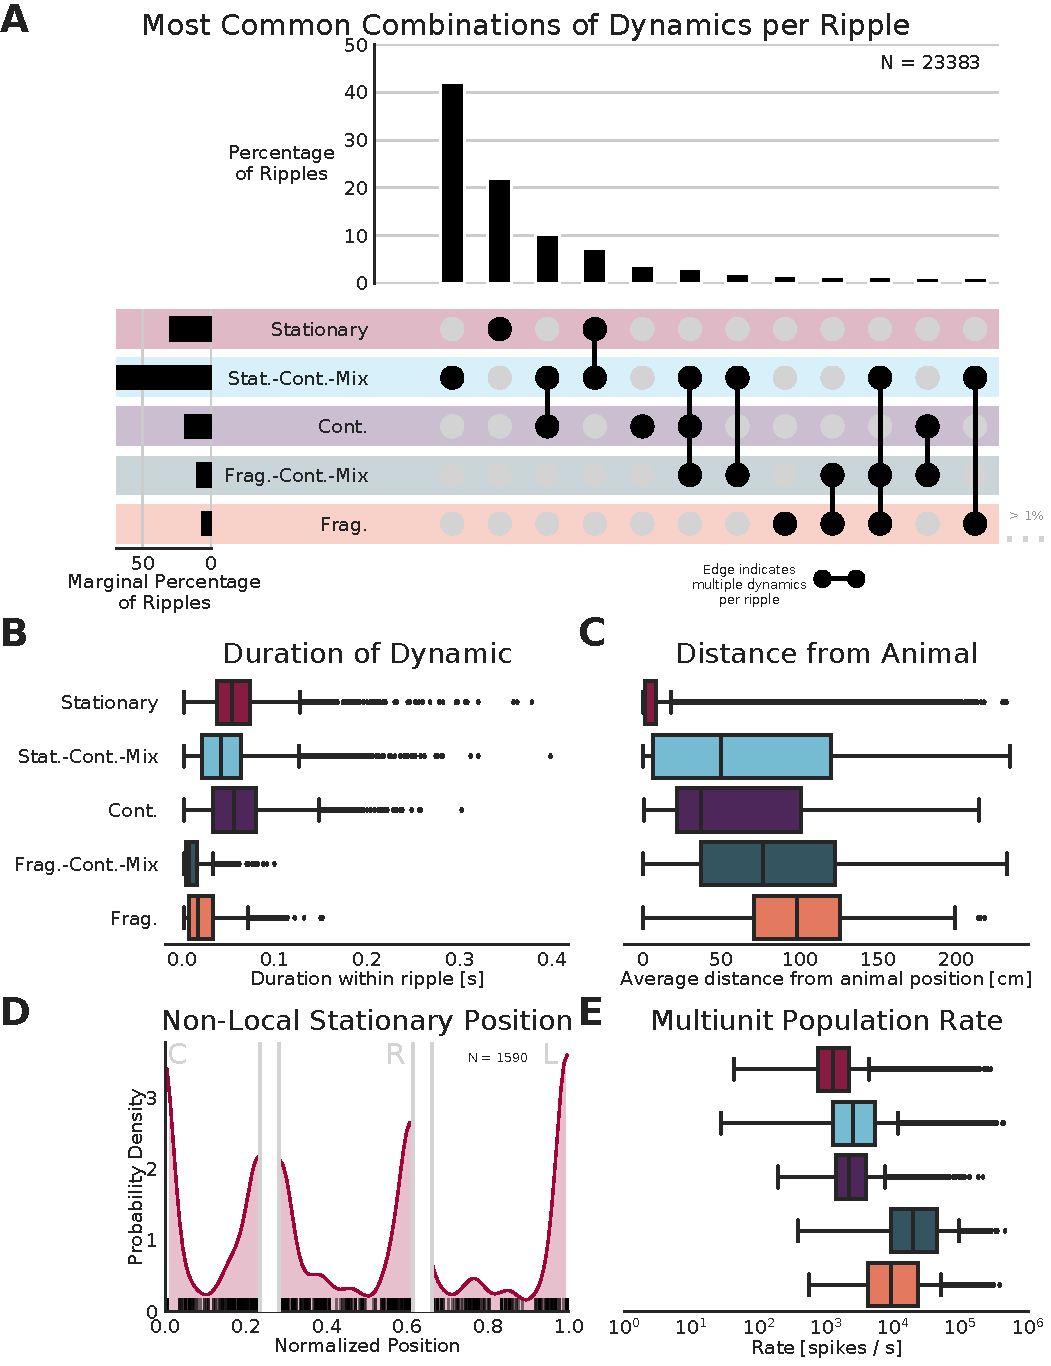
\includegraphics[width=0.80\linewidth]{figures/Figure4/Figure4_v4}
\caption{
Analysis of SWRs from all animals. \textbf{(A)} UpSet plot---which is similar to a Venn diagram with more than 3 sets---of the most common sets of dynamics within each ripple. Each row represents a possible category present in the SWR. Each column represents a set of dynamics categories, where filled-in black dots with an edge between the dots indicates that multiple categories are present in the SWR (at temporally distinct times). The sets are ordered by how often they occurred as indicated by the bar plot above each category. The total number of each category is indicated by the rotated bar plot on the left. \textbf{(B)} Distribution of the duration of each dynamic category within a SWR. \textbf{(C)} The distance of the average latent position from the animal's position for each dynamic category within each SWR. \textbf{(D)} Position of stationary trajectories on the W-track at least 30 cm away from the animal's position. \textbf{(E)} Distribution of multiunit spike rates for each dynamic category within each SWR.
}
\label{5}
\end{figure*}

We next looked at which sets of dynamics are most common. Most of the SWRs (16454 of 23382 classified SWRs or 70\%) were well described by one dynamic. Surprisingly, the most common SWRs were ones that were categorized exclusively as stationary-continuous mixtures (9860 of 23382 classified SWRs or 42\%, Figure \ref{5}A). These trajectories had a slightly shorter duration to events with continuous dynamics (median duration: stationary-continuous-mixture 72 ms vs. continuous 95 ms, Figure \ref{5}B) and occurred at a similar average distance away from the animal (mean trajectory distance from animal's position: stationary-continuous-mixture 51 cm vs. continuous 42 cm, Figure \ref{5}C). This indicates that the trajectories of these SWRs, like ones that have faster continuous dynamics, do not represent the animal's position and move at a speed that is closer to the animal's actual movement speed when running, rather than many times the animal's movement speed.

The next most common category is those SWRs that were exclusively stationary (5149 / 23382 or 22\%). Unlike the stationary-continuous mixtures, most of these trajectories represented the animal's position (Figure \ref{5}C), but there were many that represented positions as far as 226 cm from the animal. Duration. We define the ones that are more than 30 cm away from the animal as "non-local stationary trajectories". There were 1585 of 23382 classified SWRs or 7\% non-local stationary trajectories and 731 of these non-local stationary trajectories were stationary throughout the duration of the SWR. These non-local stationary trajectories represented positions all over the track, but were most common at reward wells and choice points (Figure \ref{5}D), consistent with \cite{JaiDistincthippocampalcorticalmemory2017}. The average multiunit firing rate during stationary dynamics was not lower than the other dynamics (Figure \ref{5}E.  ## Need to fix multiunit panel

\section*{Discussion}

Summary

Why our results are different from the Bayesian decoder
seek to describe all SWR events, clusterless decoding, more permissive, descriptive model

Challenges the notion that replays consist only of high speed events.

model represents middle ground between HMM and typical Bayesian decoder. allows SWR to quickly be identified because of the discrete states. Can extend to incorporate other previously experienced environments. Can work in 2D. Can precisely identify timing of dynamics because of acausal decoding

adjudicates/clarifies results of Pfiefer and Foster and Stella et al.


\begin{acknowledgements}
\end{acknowledgements}

\section*{References}
\bibliography{refs}

\onecolumn
\newpage

\section*{Methods}
\subsection*{Recording Locations and Techniques}
Ten male Long Evans rats (500-700 g, 4-9 months old) were trained on a W-track spatial alternation task. XX rats contributed to a previous study \cite{KarlssonAwakereplayremote2009}. Neural activity was recorded in CA1, CA2, CA3, MEC, Subiculum, and DG depending on the rat. We only used hippocampal tetrodes (CA1, CA2, CA3) in this study.

\subsection*{Behavioral Task}
The behavioral task is a W-track spatial alternation task as presented in \cite{KarlssonAwakereplayremote2009}. For each day, animals alternated between 15 minute sessions in a rest box and 15 minutes in the W-track. The behavioral task is a W-track spatial alternation task as presented in \cite{KarlssonAwakereplayremote2009}. For each day, animals alternated between 15 minute sessions in a rest box and 15 minutes in the W-track. Only run epochs with at least 9 hippocampal principal cells that fired at least 100 spikes were included in the analysis.

Only run epochs with at least 9 hippocampal principal cells that fired at least 100 spikes were included in the analysis.

\subsection*{Linearization}
To decrease the time it takes to run the model, the 2D position of the animal is converted into a 1D position. This is done by first defining a graph representation of the track, where edges correspond to segments of the W-track and nodes represent intersection points between those segments. Then, based on the algorithm in \cite{NewsonHiddenMarkovmap2009}, we use a Hidden Markov Model (HMM) to classify which track segment the animal is on. This algorithm was developed to track cars on roads with GPS signals. Using the HMM prevents sudden jumps from one track segment to another, which is particularly important near intersections when we are tracking the head position. Briefly, the observation model of the HMM is Gaussian and it models the likelihood of being on a track segment as the Gaussian distance to that segment with a 5 cm standard deviation. The state transition model is an empirically estimated state transition that changes with each time point that tries to ensure that the euclidean distance between successive position estimates is similar to the shortest path distance along the graph between successive position estimates. A slight bias of 0.1 is given to the diagonal to encourage staying on the same track segment. The most likely track segment the animal is on is computed using the Viterbi algorithm. After finding the track segment that corresponds to each 2D position, the 2D position is projected onto the track segment. This allows us to define a distance from the center well in terms of shortest path length on the track, where 0 cm represents the center well position. The linear distance can then be converted into a linear position by assigning each track segment a position in 1D space. The code used for linearization can be found at \url{https://github.com/Eden-Kramer-Lab/loren_frank_data_processing}.

\subsection*{SWR Detection}
Sharp wave ripples were detected using the same method as in \cite{Kayhippocampalnetworkspatial2016}. Briefly, each LFP was filtered between 150-250 Hz, squared and then summed across tetrodes--forming a single population trace over time. This trace was smoothed with a Gaussian with a 4 ms standard deviation and the square root of this trace was taken to get an estimate of the population ripple band power. Candidate SWR times were found by z-scoring the population power trace and finding times when the z-score exceeded 2 standard deviations for a minimum of 15 ms and the speed of the animal was less than 4 cm/s. The SWR times were then defined as times when the z-score was greater than the mean and contained the candidate SWR times. The code used for ripple detection can be found at \url{https://github.com/Eden-Kramer-Lab/ripple_detection}.

\subsection*{Spike Sorting}

\subsection*{Simulated Data}

\subsection*{The Model}

\subsection*{Encoding - Clusterless}
In order to encode how each tetrode's unsorted spiking activity relates to position, we use a marked point process framework. For each multiunit spike during movement (defined as time periods when the running speed is greater than 4 cm/s), the associated waveform features (the marks) and position are recorded in a (n-spikes, n-features + n-position-dimensions) array. In our case, the waveform features correspond to the max amplitude observed on each tetrode wire at the time of the multiunit spike. This array is used as the training samples in a kernel density estimator during the decoding step.

\subsection*{Encoding - Sorted Spikes}
In order to encode how each cell's spiking activity relates to position (the place field), we fit a generalized linear model (GLM) with a Poisson response distribution to each cell's spiking activity during movement (defined as time periods when the running speed is greater than 4 cm/s). We estimate the parameters $\beta$, which consist of $\beta_{0}$, the average firing rate over time, and $\beta_{i}$, weights for third degree B-splines basis functions $f_{i}$ over position (or tensor products of the B-splines when position is two dimensional). B-spline basis functions are used because place field firing activity is assumed to vary smoothly over position and this prior knowledge can be exploited to reduce the total number of model parameters needed. Each basis function is spaced every 5 cm over the range of the position and zero constrained so that the change encoded by the parameters is relative to the baseline firing rate. We use a log link function to convert the linear combination of parameters to an instantaneous firing rate over time $\lambda(t)$ to ensure the rate is always positive. 

$$log(\lambda(t)) = \beta_{0} + \sum_{i} f_{i}(position)\beta_{i}$$

A small L2 penalization term $-\lambda\norm{\beta_{i}}_{2}^{2}$ used to prevent model fitting instability when spiking activity is very low. We set this to 0.5 for all cells. Fitting is done by maximizing the penalized likelihood using a Newton-Raphson algorithm.

\subsection*{Decoding - Clusterless}

\subsection*{Classification of Dynamics}
We used a threshold of 0.8 to classify the probability of each state into 5 categories. Time periods during sharp wave ripples are labeled as Stationary, Continuous, or Fragmented when the probability of each state is above 0.8. Time periods are labeled as Stationary-Continuous-Mix or Fragmented-Continuous-Mix when the sum of Stationary and Continuous or Fragmented and Continuous are above 0.8, respectively. Time periods where none of these criterion are met are considered unclassified because there is not an interpretation for all three dynamics being equally likely.

\subsection*{Replay distance from animal}
Replay distance from the animal is defined as the shortest path distance along the track graph between the animal's projected position on the track graph (see Linearization) and the MAP estimate of the joint posterior marginalized over state, which is defined as the center of the position bin with the greatest posterior value.

\subsection*{Software and Code availability}
Python code used for analysis and generating figures in the paper is available at: \url{https://github.com/Eden-Kramer-Lab/replay_trajectory_paper}. Code for the classifier is available in a separate software repository to facilitate code reuse at: \url{https://github.com/Eden-Kramer-Lab/replay_trajectory_classification}. All code is open-source and licensed under the MIT Software License. Classifier code can be easily installed as a python package with all requisite dependencies using pip or conda. See software repositories for specific details.

\newpage

%%%%%%%%%%%%%%%%%%%%%%%%%%%%%
% Supplementary Information %
%%%%%%%%%%%%%%%%%%%%x%%%%%%%%%
\beginsupplement
\captionsetup*{format=largeformat}

\begin{figure*}%[tbhp]
\centering
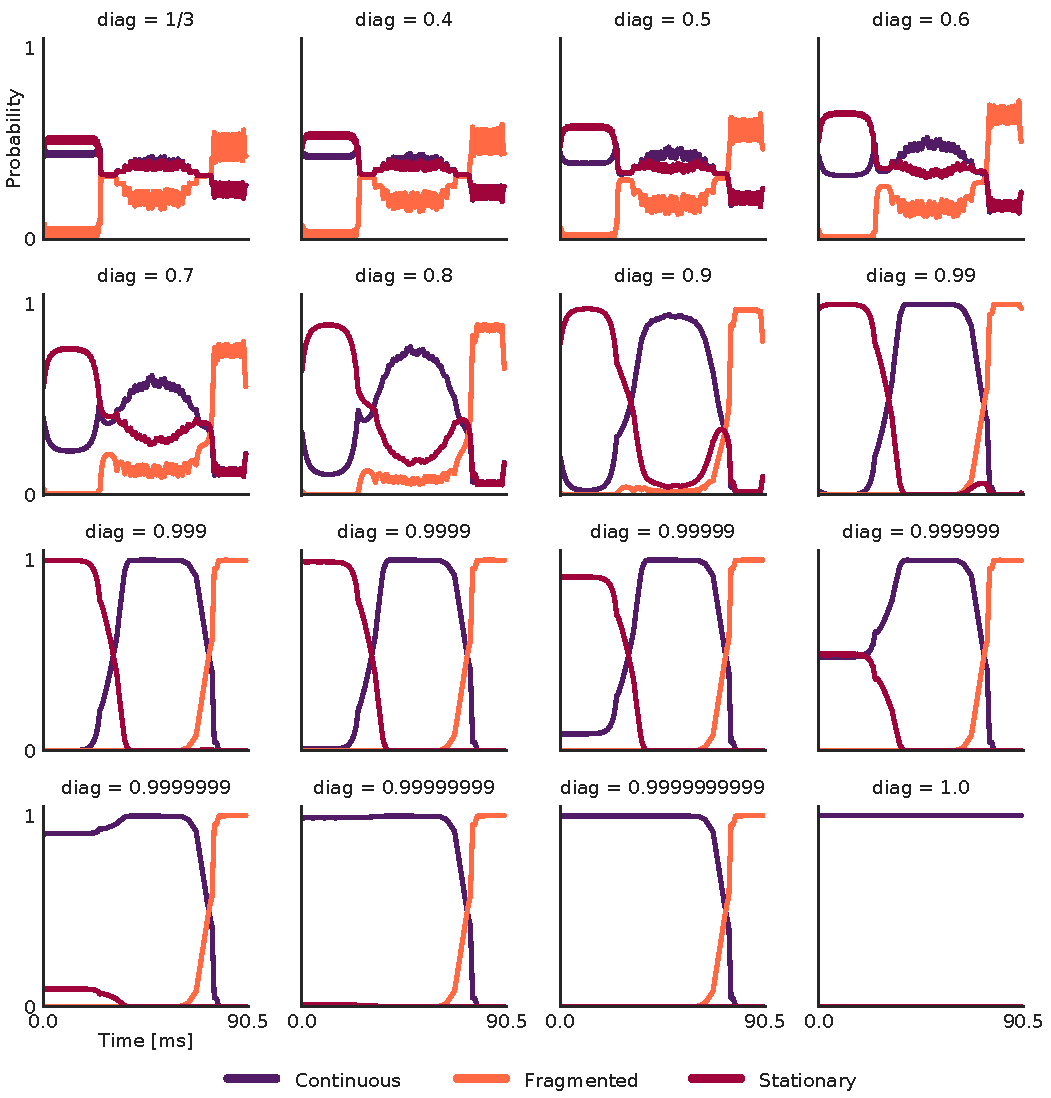
\includegraphics[width=0.80\linewidth]{figures/Figure1-supplemental1/Figure1_v2_supplemental1}
\caption{The model is robust to changes in the discrete transition matrix. Each plot shows the probability of each dynamic on simulated data example from Figure 1 with a different diagonal value--which governs the probability of remaining in that state. The off-diagonal values--the probability of switching to one of the other dynamics--are set to be equally likely with the remainder of the probability, as in Figure 1D. The first plot (upper left) shows the case when all dynamics are equally likely. The diagonal increases from left to right, top to bottom, until the case where the diagonal is one and the off-diagonal is zero--i.e. the case where there is no probability of switching to another state.}
\label{fig:Figure1-Figure supplement 1}
\end{figure*}

\begin{figure*}%[tbhp]
\centering
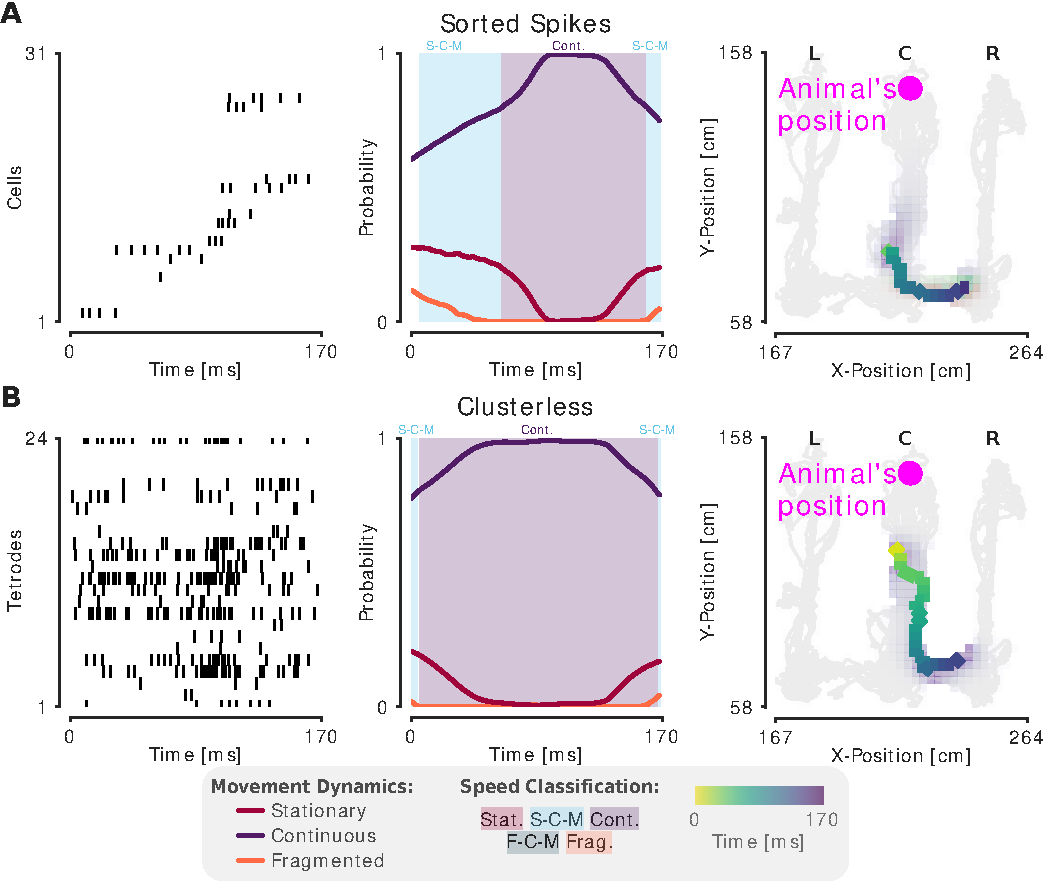
\includegraphics[width=0.80\linewidth]{figures/Figure2-supplemental1/Figure2_v3-supplemental1}
\caption{Decoding the same SWR in Figure 2 using 2D clusterless and sorted spikes. \textbf{(A)} The left plot shows the spikes from cells arranged by the linear position of the peak of place field as in Figure 2. The middle plot shows the probability of each dynamic over time from the 2D decode. Shaded regions indicate classification category as in Figure 1G and 2. The rightmost plot shows the MAP estimate of the latent position with color indicating time. The latent position posterior summed over time is shown in purple underneath. The light grey lines represent the position of the animal over the entire epoch and the red dot represents the animal's position. \textbf{(B)} Same as in A, but with clusterless decoding.}
\label{fig:Figure2-Figure supplement 1}
\end{figure*}

\begin{figure*}%[tbhp]
\centering
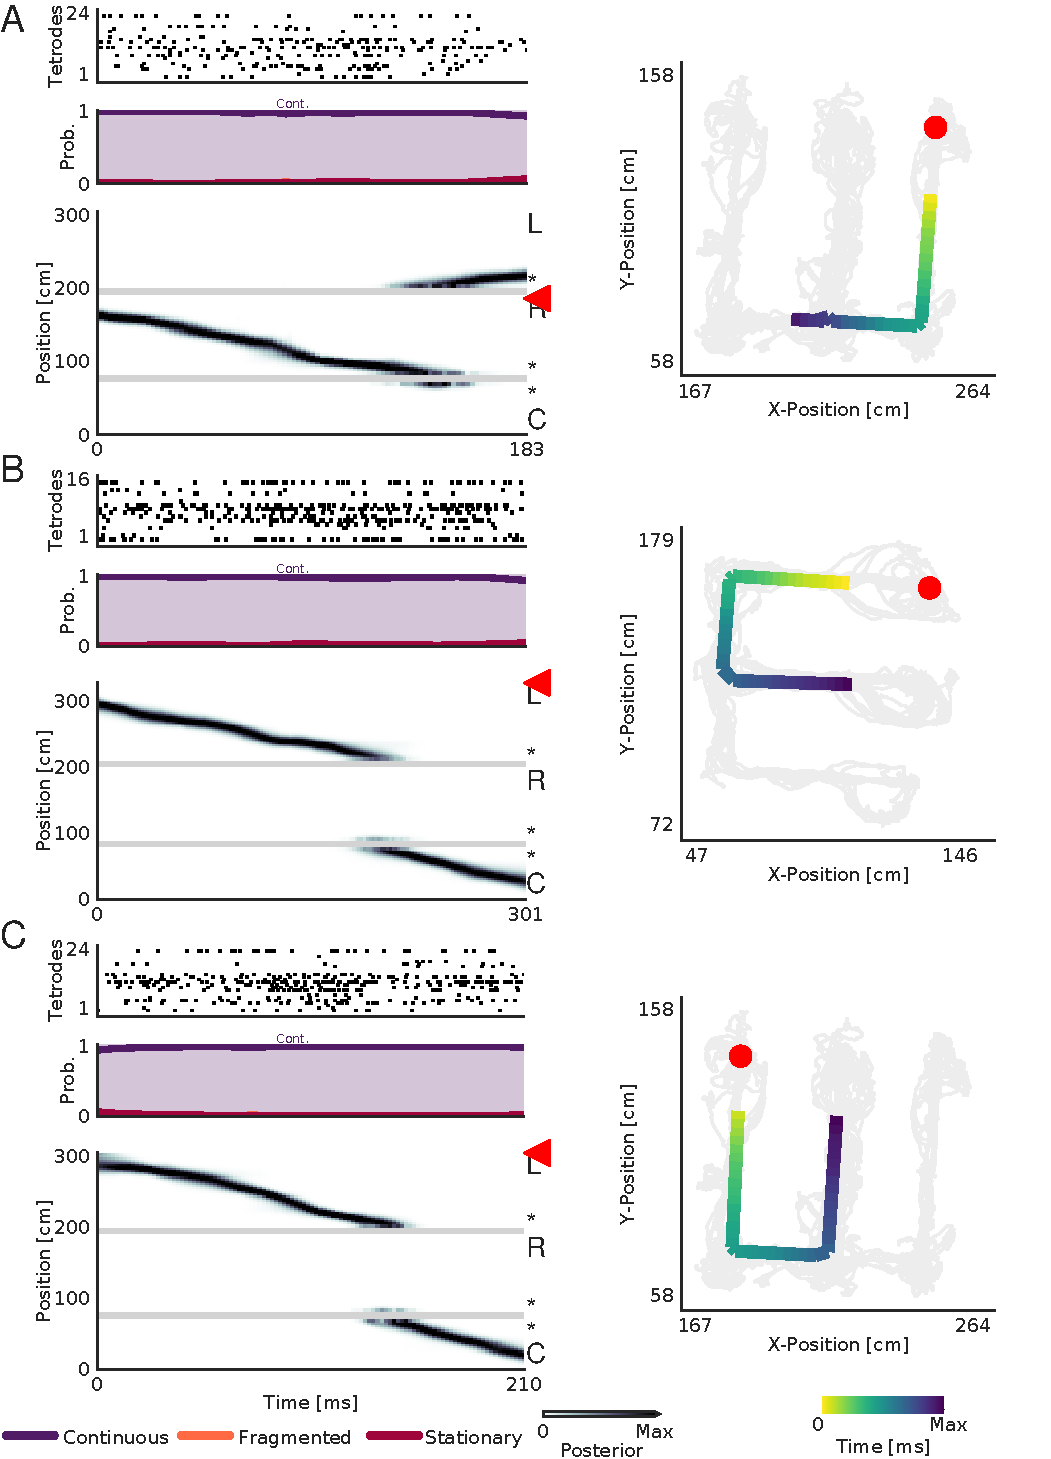
\includegraphics[width=0.80\linewidth]{figures/Figure2-supplemental2/Figure2_v3-supplemental2}
\caption{A-C. Examples of continuous replays. Left panel uses the same conventions as Figure 2A and 2B. Right panel shows the 1D MAP estimate projected back to 2D as in Figure 2C. Color indicates time. Light grey lines indicate the animal's position over the entire epoch.}
\label{fig:Figure2-Figure supplement 2}
\end{figure*}

\begin{figure*}%[tbhp]
\centering
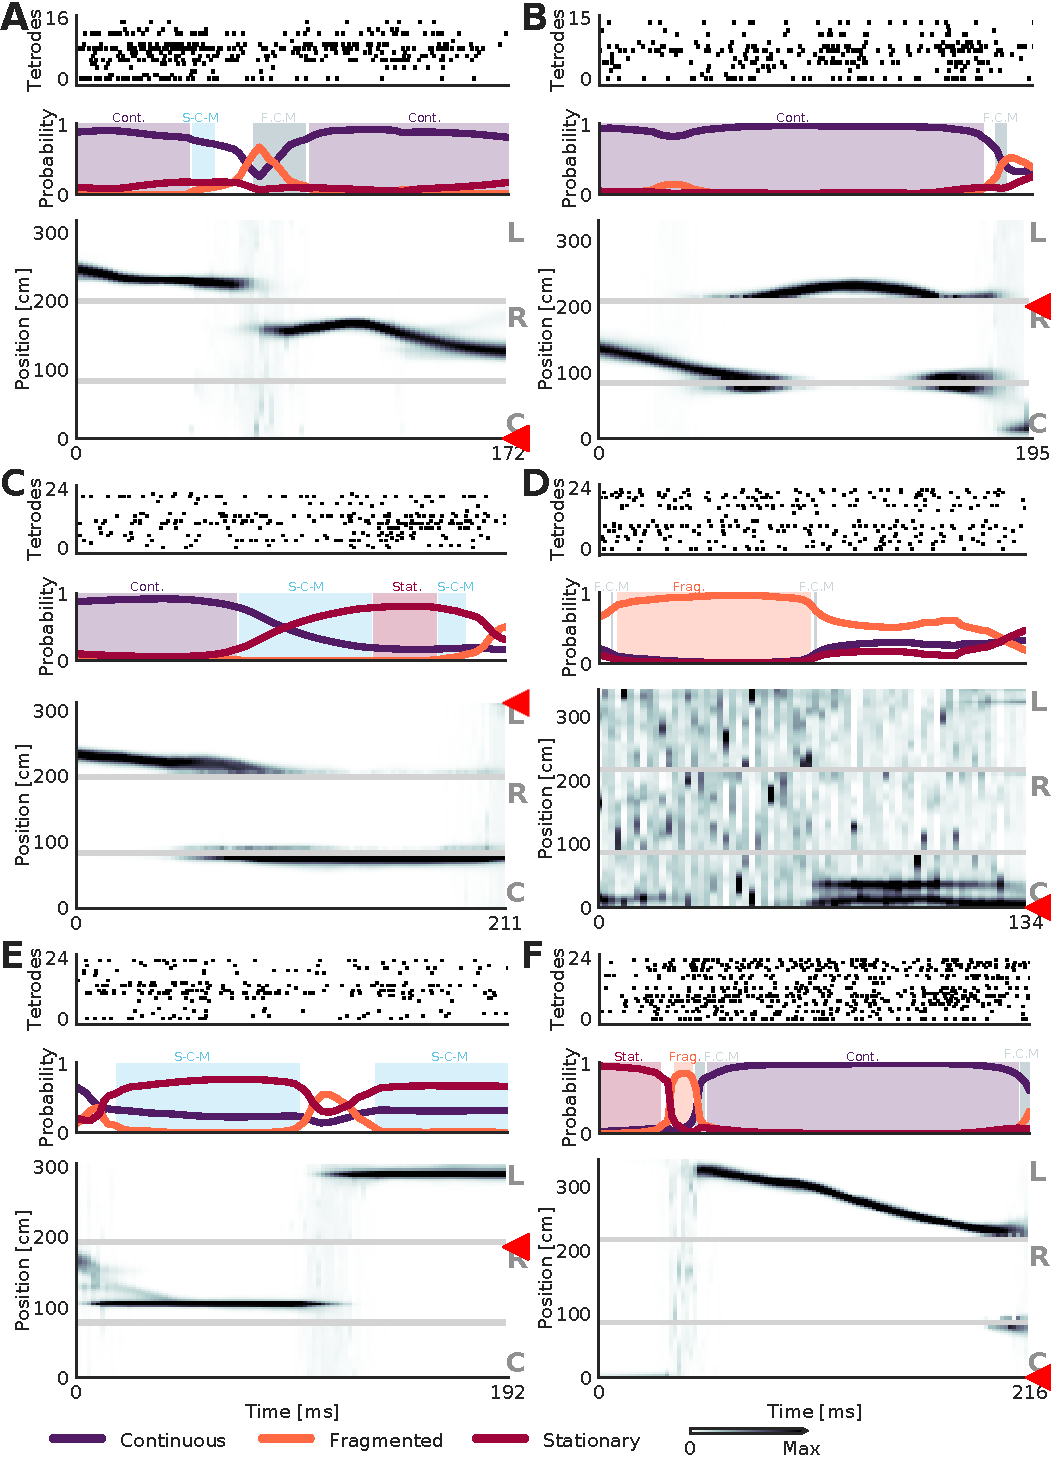
\includegraphics[width=0.80\linewidth]{figures/Figure3-supplemental1/Figure3_v3_supplemental1}
\caption{More examples of replays that would not be well-characterized by using the Bayesian decoder. Conventions are the same as in Figure 3. \textbf{(A)} A continuous replay that starts in the left arm back toward the center well, jumps to the right arm and continuous back toward the center well. \textbf{(B)} A continuous replay that travels down the right arm toward the center well, proceeds past the choice point toward the left well and then returns back to the choice point. \textbf{(C)} A replay that starts down the left arm toward the center arm and turns into a stationary trajectory near the choice point. \textbf{(D)} The first half is a fragmented replay and the second half is unclassified. \textbf{(E)} A stationary trajectory in the first half of the SWR on the right arm and then a stationary trajectory in the SWR at the left well. \textbf{(F)} A stationary trajectory that starts at the animal's position at the center well, then jumps to the left well and comes back toward the center well.
}
\label{fig:Figure3-Figure supplement 1}
\end{figure*}

\begin{figure}%[tbhp]
\centering
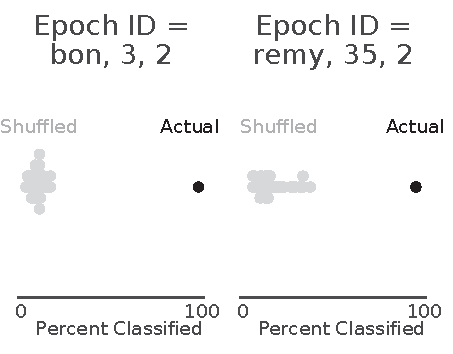
\includegraphics[width=0.80\linewidth]{figures/Figure5/Figure5_v1}
\caption{Comparison of real vs. position shuffled data for two epochs from different animals. Line represents the percent of SWR classified in that epoch for real data. The histogram represents the distribution after 50 shuffles of the position data. Position data was shuffled by resampling with replacement from the set of all observed positions in that epoch, destroying position information but preserving spiking timing.}
\label{Figure3-Figure supplement 2}
\end{figure}

%TC:endignore
%the command above ignores this section for word count

\end{document}
